\documentclass{standalone}
\usepackage{amsmath}
\usepackage{pgfplots}
\pgfplotsset{compat=1.16}
\usepgfplotslibrary{groupplots}
\usetikzlibrary{math}
\usetikzlibrary{calc}
\usetikzlibrary{arrows.meta}
\begin{document}

\pgfplotsset{
    width=0.95\textwidth,
    scale only axis,}
		
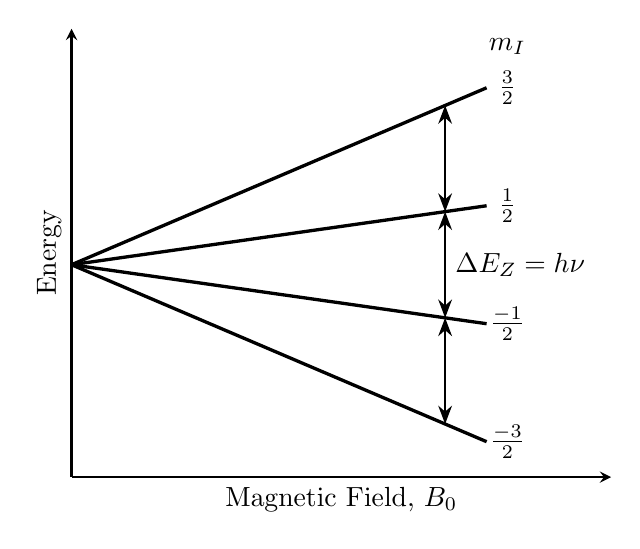
\begin{tikzpicture}
	\begin{axis}[
		axis lines = {left},
		smooth,
		thick,
		xlabel = {Magnetic Field, $B_0$}, 
		ylabel = Energy, 
		ticks = none,
		no markers, 
		xmin=0, xmax=13,
		ymin=-18, ymax=20,
		scale=1.0]

		\pgfplotsinvokeforeach{0,...,3}{
			\addplot [very thick, black, samples=50, domain=0:10] {(#1 - 3/2) * x};
			\node (#1) at (axis cs: {10.5},{10*(#1-3/2)}) {\(\frac{\pgfmathparse{int(2*#1-3)} \pgfmathresult}{2}\)};
		}

		% Annotation lines and arrows
		\pgfplotsinvokeforeach{0,...,2}{
			\draw[Stealth-Stealth] (axis cs: {9},{9*(#1-3/2)}) -- (axis cs: {9},{9*(#1-1/2)});
		}

		\node[right]	(Ez)	at	(axis cs: {9},{0})	[align=left]{$\Delta E_{\mathup{Z}} = h \nu$};
		\node (mS) at (axis cs: {10.5},{18.5}) {\(m_I\)};
	\end{axis}
\end{tikzpicture}	
\end{document}
